\documentclass[a4paper, 20pt, openany]{book}
\usepackage{titlesec}
\titleformat{\chapter}[display]   
{\normalfont\huge\bfseries}{\chaptertitlename\ \thechapter}{20pt}{\Huge}   
\titlespacing*{\chapter}{5pt}{-50pt}{40pt}
\usepackage{ucs}
\usepackage[utf8x]{inputenc}
\usepackage{enumitem}
\usepackage{a4wide}
\usepackage{geometry}
\usepackage[automark]{scrpage2}
\pagestyle{scrheadings}
\usepackage{amssymb}
\usepackage{ulem}
\usepackage[doublespacing]{setspace}
\usepackage[procnames]{listings}
%\usepackage{color}
\usepackage[pdftex]{graphicx,color}
\usepackage{textcomp}
\usepackage{titlesec}
\titleformat*{\section}{\large\bfseries}
\clearscrheadfoot
\ohead{Informatik II Skript - Steffen Lindner}
\cfoot{\pagemark}
\geometry{a4paper,left=10mm,right=10mm, top=10mm, bottom=2cm} 
\parindent0pt

\author{Steffen Lindner}
\title{\vspace{-2cm}Informatik II Skript}
\date{\today{}}
\lstdefinelanguage{Scheme}{
  morekeywords=[1]{define, define-syntax, define-macro, lambda, define-stream, stream-lambda},
  morekeywords=[2]{begin, call-with-current-continuation, call/cc,
    call-with-input-file, call-with-output-file, case, cond,
    do, else, for-each, if,
    let*, let, let-syntax, letrec, letrec-syntax,
    let-values, let*-values,
    and, or, not, delay, force,
    quasiquote, quote, unquote, unquote-splicing,
    map, fold, syntax, syntax-rules, eval, environment, query },
  morekeywords=[3]{import, export},
  alsodigit=!\$\%&*+-./:<=>?@^_~,
  sensitive=true,
  morecomment=[l]{;},
  morecomment=[s]{\#|}{|\#},
  morestring=[b]",
  basicstyle=\small\ttfamily,
  keywordstyle=\bf\ttfamily\color[rgb]{0,.3,.7},
  commentstyle=\color[rgb]{0.133,0.545,0.133},
  stringstyle={\color[rgb]{0.75,0.49,0.07}},
  upquote=true,
  breaklines=true,
  breakatwhitespace=true,
  literate=*{`}{{`}}{1}
}

\lstset{language=Scheme}

\begin{document}



        
\maketitle
\tableofcontents

\chapter{Einführung - 14.04.15}\uline{Scheme}: Ausdrücke, Auswertung und Abstraktion 

\uline{Dr.Racket}: Definitionsfenster (oberer Bereich), Interaktionsfenster (unterer Bereich) 

Die Anwendung von Funktionen wird in Scheme \uline{ausschließlich} in \uline{Präfixnotation} durchgeführt.

\paragraph{Beispiele}
\begin{flushleft}
	\begin{tabular}{c|c}
		Mathematik & Scheme \\
		44-2 & (- 44 2) \\
		f(x,y) & (f x y) \\
		$\sqrt{81}$& (sqrt 81) \\
		9² & (expt 9 2) \\
		3! & (! 3)  {}
	\end{tabular}
\end{flushleft}

Allgemein: ($<function> <arg1> <arg2> ...$)

(+ 40 2) und (odd? 42) sind Beispiele für \uline{Ausdrücke}, die bei \uline{Auswertung} einen Wert liefern. (Notation: $\rightsquigarrow$)

(+ 40 2) $\rightsquigarrow$ 42 ($\rightsquigarrow$ = Auswertng / Reduktion / Evalutation)

(odd? 42) $\rightsquigarrow$ \#f

Interaktionsfenster: Read $\rightarrow$ Eval $\rightarrow$ Print $\rightarrow$ Read ... (Read-Eval-Print-Loop aka. REPL)

\uline{Literale} stehen für einen konstanten Wert (auch konstante) und sind nicht weiter reduzierbar.

Literal: 

\#t, \#f (true, false, Wahrheitswerte) (boolean) \\
"abc", "x", " " (Zeichenkette) (String) \\
0 1904 42 -2 (ganze Zahlen) (Integer) \\
0.42 3.1415 (Fließkommazahl) (Reel) \\
1/2, 3/4 (rationale Zahl) (Rational) \\
$\backslash\_('')\_/"$ (Bilder) (Image)

\chapter{Ausdrücke, Defines, usw. - 16.04.2015}

Auswertung \uline{zusammengesetzter Ausdrücke} in mehreren Schritten (steps), von "innen nach außen" bis keine Reduktion mehr möglich ist.

\begin{center}
(+ (+ 20 20) (+ 1 1)) $\rightsquigarrow$ (+ 40 (+ 1 1) $\rightsquigarrow$ (+ 40 2) $\rightsquigarrow$ 42
\end{center}

\uline{Achtung}: Scheme rundet bei Arithmetik mit Fließkommazahlen (interne Darstellung ist binär).

Bsp.: Auswertung des zusammengesetzten Ausdrucks 0.7 + (1/2)/0.25 - 0.6/0.3

Arithmetik mit rationalen Zahlen ist exakt.

Ein Wert kann an einen \uline{Namen} (auch Identifier) gebunden werden , durch

\begin{center}
(define $<id>$ $<e>$) ($<id>$ Identifier, $<e>$ Expression)
\end{center}

Erlaubt konsistente Wiederverwendung und dient der Selbstdokumentation von Programmen.

\uline{Achtung}: Dies ist eine sogenannte \uline{Spezifikation} und kein Ausdruck. Insbesodnere besitzt diese Spezialform \uline{keinen} Wert, sondern einen Effekt: Name $<id>$ wird an den Wert von $<e>$ gebunden.



Namen können in Scheme fast beliebig gewählt werden, solange:

\begin{enumerate}
\item die Zeichen (kommt noch) nicht vorkommen
\item der Name nicht einem numerischen Literal gleicht
\item kein whitespace (Leerzeichen, Tabulatoren, Return) enthalten ist.
\end{enumerate}

Bsp.: euro $\rightarrow$ us$\$$

\uline{Achtung}: Groß-/Kleinschreibung ist in Identifiern nicht relevant.

Eine \uline{Lambda-Abstraktion} (auch: Funktion, Prozedur) erlaubt die Formulierung von Ausdrücken, die mittels \uline{Parametern} konkreten Werten abstrahieren:

\begin{center}
(lambda ($<p1> <p2> ...$) $<e>$), $<e>$ Rumpf
\end{center}

$<e>$ enthälft Vorkommen der Parameter $<p1>,<p2>$...

(lambda ...) ist eine Spezialform. Wert der Lambda-Abstraktion ist $\#<procedure>$

\uline{Anwendung} (auch: Applikation/Aufruf) der Lambda-Abstraktion führt zur Ersetzung der vorkommenden Parameter im Rumpf durch die angegebenen \uline{Argumente}: 

(lambda (days) (* days (* 155 min-in-a-day))) $\rightsquigarrow$ (* 365 (* 155 min-in-a-day)) $\rightsquigarrow$ 81468000

In Scheme leitet ein Semikolon einen \uline{Kommentar}, der bis zum Zeilenende reicht, ein und wird vom System bei der Auswertung ignoriert.

Prozeduren sollten im Programm eine ein-bis zweizeiliger Kurzberschreibung direkt voran gestellt werden.



\chapter{Signaturen, Testfälle - 21.04.15}
Eine \underline{Signatur} prüft, ob ein Name an einen Wert einer angegebenen Sorte (Typ) gebunden wird. Signaturverletzungen werden protokolliert.

\begin{center}
$(: \ <id>  \ <signatur>)$
\end{center}

Bereits eingebaute Signaturen:

\begin{itemize}
\item natural $\mathbb{N}$
\item integer $\mathbb{Z}$
\item rational $\mathbb{Q}$
\item real $\mathbb{R}$
\item number $\mathbb{C}$
\item boolean
\item string
\item image
\end{itemize}

(: ...) ist eine Spezialform ohne Wert, aber Effekt: Signaturprüfung \\

\underline{Prozedur-Signaturen} spezifizieren sowohl Signaturen für die Parameter p1, p2, ... , pn als auch den Ergebniswert der Prozedur:

\begin{center}
$(<signatur p_{1}> ... <signatur p_{n}> -> <signatur-ergebnis>)$
\end{center}

Prozedur-Signaturen werden \underline{bei jeder Anwendung} eine Prozedur auf Verletzung geprüft. \\


\underline{Testfälle} dokumentieren das erwartete Ergebnis einer Prozedur für ausgewählte Argumente:

\begin{center}
$(check-expect <e_{1}> <e_{2}>)$
\end{center}

Werte Ausruck $<e_{1}>$ aus und teste, ob der erhaltene Wert der Erwarung (= der Wert von $<e_{2}>$) entspricht. \\

Einer Prozedurdefinition sollten Testfälle direkt vorangestellt werden.

Spezialform: Kein Wert, aber Effekt: Testverletzung protokollieren.\\

\underline{Konstruktionsanleitung für Prozeduren}
\begin{itemize}
\item ; ... (1) Kurzbeschreibung (1-2 zeiliger Kommentar mit Bezug auf Parameter)
\item (: ...) (2) Signatur
\item (check-expect ...) (3) Testfälle
\item (define (lambda (...) ...) (4) Prozedur + Rumpf
\end{itemize}

\underline{Top-Down-Entwurf} (Programmieren durch "Wunschdenken") 

Bsp.: Zeichen Ziffernblatt (Stunden- und Minutenzeiger) zur Uhrzeit H:m auf einer analogen 24h-Uhr 
\begin{itemize}
\item Minutenzeiger legt 360°/60 pro Minute zurück (360/60 * m)
\item Stundenzeiger legt 360°/12 pro Stunde zurück (360/12 * h + 360/12 * m/60)
\end{itemize}

\chapter{Substitutionsmodell, Fallunterscheidung - 23.04.15}
\underline{Reduktionsregeln} für Scheme (Fallunterscheidug je nach Ausrucksart)

Wiederhole, bis keine Reduktion mehr möglich:
\begin{itemize}
\item Literal (1, "abc", \#t, ...) [eval$_{lit}$]

l $\rightsquigarrow$ l
\item Identifier id (pi, clock-face, ...) [eval$_{id}$]

id $\rightsquigarrow$ gebundener Wert
\item Lambd-Abstraktion 

(lambda () ) $\rightsquigarrow$ (lambda () ) [eval$_{\lambda}$]

\item Applikation (f, e1, e2)
 \begin{itemize}
 \item (1) f, e1, e2 reduziere, erhalte f', e1', e2' 
 \item (2)
   \begin{itemize}
   \item Operation f' auf e1', e2', ... falls f' primitive Operation (+, *, ...) [apply$_{prim}$]
   \item Argumentenwert e1', e2', ... Rumpf von f' einsetzen, dann Rumpf reduzieren , falls f' Lambdaabstraktion [apply$_{\lambda}$]
   \end{itemize}
 \end{itemize}
\end{itemize}

\underline{Beispiel:} Applikation

(+ 40 2)

$\rightsquigarrow$ (\#$<$ procedure + $>$ 40 2) $\rightsquigarrow$ 42

eval$_{lit}$ (+)

eval$_{lit}$ (40)

eval$_{lit}$ (2)\textsl{•}


(position-minute-hand 30)

$\rightsquigarrow$ ((lambda (m) (* degrees-per-minute m)) 30)

$\rightsquigarrow$ (* degrees-per-minute 30)

$\rightsquigarrow$ (* degress-per-minute 30)

$\rightsquigarrow$ (\#$<$procedure * $>$ 360/60 30)

Bezeichnen (lambda (x) (* x x )) und (lambda (r) (* r r)) die gleiche Prozedur? $\Rightarrow$ Ja!

\underline{Achtung}: Das hat Einfluss auf das korrekte Einsetzen von Argumenten für Parameter! (s. apply$_{\lambda}$)

Das \underline{bindenen Vorkommen} eines Identifiers x kann im Programmtext systematisch bestimmt werden: suche strik von "innen nach außen" bis zum ersten 

\begin{itemize}
\item (lambda (x) )
\item (define x )
\end{itemize}

(Prinzip der \underline{lexikalischen Bindung})

Übliche Notation in der Mathematik: \underline{Fallunterscheidung}

$ maximum(x_{1}, x_{2})=\left\{\begin{array}{cl} x_{1}, & \mbox{falls } x_{1} \geq x_{2}\\ x_{2}, & \mbox{sonst} \end{array}\right. $

\underline{Tests} auch (Prädikate) sind Funktionen, die einen Wert der Signatur boolean liefern. Typische primitive Tests:

\begin{itemize}
\item (: = (number number $\rightarrow$ boolean))
\item (: $<$ (real real $\rightarrow$ boolean)), auch $>, \le, \geq$
\item (: string=? (string string $\rightarrow$ boolean)), auch string$>$?, string$\le$?
\item (: boolean? (boolean boolean $\rightarrow$ boolean))
\item (: zero? (number $\rightarrow$ boolean))
\item odd?, even?, positive?, negative?, ...
\end{itemize}

Binäre Fallunterscheidung: \underline{if}

(if $<t_{1}> <e_{1}> <e_{2}>$) \\

Mathematisch: 
$ \left\{\begin{array}{cl} e_{1}, & \mbox{falls } t_{1}\\ e_{2}, & \mbox{sonst} \end{array}\right. $

\chapter{One-of Signatur - 28.04.15}
Die Signatur \underline{one-of} lässt genau einen der aufgezählten n Werte zu: 
\begin{center}
	(one-of $<e_1> ... <e_n>$)
\end{center}

Reduktion von if: \\

(if $t_{1}\  e_{1}  \ e_{2}$) $ \rightsquigarrow$ 
$ \left\{\begin{array}{cl} <e_{1}>, & \mbox{falls t1' = \#t ; e2 wird niemals ausgewertet} \\ <e_{2}>, & \mbox{sonst; e1 wird niemals ausgewertet} \end{array}\right. $ \\



(1) Reduziere $t_{1}$, erhalte $t_{1}'$ \\

Spezialform Fallunterscheidung (conditional expression):
\begin{center}
(cond ($<t_1 > <e_1 >$) ... ($<t_n > <e_n >$) (else $<e_{n+1}>$)) (else optional)
\end{center}

Werte die Tests in der Reihenfolge $t_{1},t_{2},...,t_{n}$ aus. Sobald $t_i $ \# t ergibt werte Zweig $e_i $ aus. $e_i $ ist das Ergebnis der Fallunterscheidung. Wenn $t_n $ \# f liefert, dann liefere
\begin{center}
$ \left\{\begin{array}{cl} Fehlermeldung, & \mbox{"cond: alle Tests ergaben \#f", falls kein else-Zweig \ } \\ <e_{n+1}>, & \mbox{sonst} \end{array}\right. $
\end{center}

Reduktion von cond [eval$_{cond}$]

\begin{center}
	(cond ($<t_{1}> <e_{1}>) (<t_2> <e_2>) ...$) $\rightsquigarrow    \left\{\begin{array}{cl} <e_{1}>, & \mbox{falls t1' = \#f} \\ (cond (<t_{2}> <e_{2}> ) (...) ), & \mbox{sonst} \end{array}\right. $
\end{center}

Reduziere $t_1$, erhalte $t_1$'.

(cond ) $\rightsquigarrow$ Fehlermeldung "Alle Tests..."

(cond (else $<e_{n+1}>$)) $\rightsquigarrow$ $e_{n+1}$

cond ist "systematischer Zucker" \\
(auch: abgleitete Form) für eine verschachtelte Anwendung von 'if':

(cond ($<t_1> <e_1>$) ($<t_1> <e_1>$) ... ))) entspricht (if $<t_1> <e_1> (if <t_1> <e_1> (if ...)$)

Spezialformen 'and' und 'or':
\begin{center}
$(or <t_!> <t_2> ... <t_n>)$ entspricht $(if <t_1> \#t (or <t_2> ...)$)

(or) $\rightsquigarrow$ \#f
\end{center}
\begin{center}
$(and <t_1>...<t_n> \rightsquigarrow (if <t_1> (and <t_2> ... <t_n>) \#f$)

(and) $\rightsquigarrow \# t$
\end{center}

\chapter{Zusammengesetzte Daten - 30.04.15}
Ein Charakter \underline{besteht aus} drei \underline{Komponenten}.
\begin{itemize}
  \item Name des Charakters (name)
  \item Handelt es sich um einen Jedi? (jedi?)
  \item Stärke der Macht (force)
\end{itemize}

$\rightarrow$ \underline{Datendefinition} für zusammengesetzte Daten.

Konkreter Charakter: \\

\begin{tabular}{c|c}
Name & "Luke Skywalker" \\ \hline
jedi? & \#f \\ \hline
force & 25 \\
\end{tabular}\\

; Ein Charakter (character) besteht aus \\
; - Name (name)\\
; - Jedi-Status (jedi?)\\
; - Stärke der Macht (force)\\

\begin{center}
(define-records-procedures charakter

make-character

character?

(character-name

character-jedi

character-force))
\end{center}

(make-character n j f) $\rightsquigarrow$ $<records>$ (konstruktion)

(character-name $<record>$ $\rightsquigarrow$ n (Komponentenzugriff)

(character-jedi? $<record>$) $\rightsquigarrow$ j (Komponentenzugriff)

(character-force $<record>$) $\rightsquigarrow$ f (Komponentenzugriff)

Zusammengesetzte Daten = \underline{Records} in Scheme.

Record-Definition legt fest:

\begin{itemize}
  \item Record-Signatur
  \item \underline{Konstruktor} (Baut aus Komponenten einen Record)
  \item Prädikat (liegt Record vor?)
  \item Liste von \underline{Selektoren} (lesen jewils eine Komponenten des Records)
\end{itemize}

\begin{center}
(define-records-procedures $<t>$

make-$<t>$ ; Konstruktor

$<t>$?

($<t>-<comp_1> ...<t>-<comp_n>4))$ ; Liste der n-Seleketoren
\end{center}

Verträge des Konstruktors / der Selektoren für Record-Signatur $<t>$ mit n Komponenten namens $<comp_1> ... <comp_n>$:

\begin{itemize}
  \item (: make-$<t>$ ($<t_1>...<t_n> \rightarrow <t>$))
  \item (: $<t>-<comp_1> (<t> \rightarrow <t_1>$))
  \item ...
  \item (: $<t>-<comp_n> (<t> \rightarrow <t_n>$))
\end{itemize}

Es gilt für die Strings n, Booleans j und Integer f:

(character-name (make-character n j f)) = n 

(analog für den Rest)

Interaktion von Funktionen (\underline{algebraische Eigenschaften}).

Spezialform \underline{check-property}:

\begin{lstlisting}
(check-property
  (for-all ((<id_1>  <sig_1> ... <id_n>  <sig_n>))
  <e>))
\end{lstlisting}
$<e>$ bezieht sich auf $<id_1>... <id_n>$.

Test erfolgreich, falls $<e>$ für bel. gewählte Bindungen für $<id_1>...<id_n>$ immer \#t ergibt.

Interaktion von Selektor und Konstruktor:

\begin{lstlisting}
(check-property  
  (for-all ((n string)
            (j booleans)
            (f integer))
  (string=? (character-name (make-character n j f)) n )))
\end{lstlisting}

\underline{Beispiel:} Die Summe zweier natürlicher Zahlen ist mindestens so groß wie jede dieser Zahlen: $\forall x_1, x_2 \in \mathbb{N} : x_1 + x_2 \geq max \ {x_1, x_2}$

\begin{lstlisting}
(check-property
  (for-all ((x_1 natural)
            (x_2 natural))
  (\geq (+ x_1 x_2) (max x_1 x_2))))
\end{lstlisting}

Konstruktion von Funktionen, die zusammengesetzte Daten \underline{konsumieren}:

\begin{itemize}
  \item Welche Record-Komponenten sind relevant für Funktionen?
  
  $\rightarrow$ Schablone:
  
  ; könnte Charakter e ein Sith-Lord sein?
  
  (: sith? (character $\rightarrow$ boolean))
  
  \begin{lstlisting}
  (define sith?
    (lambda (e) 
      ... (character-jedi? c) ... (character-force c) ... ))
  \end{lstlisting}
\end{itemize}

Konstrukton von Funktionen, die zusammengesetzte Daten \underline{konstruieren}: 

\begin{itemize}
  \item Der Konstruktor \underline{muss} aufgerufen werden.
  
  $\rightarrow$ Schablone:
  
  \begin{lstlisting}
  (define    
    (lambda (...)
      (make-<t> ...) ...))
  \end{lstlisting}

\end{itemize}

\chapter{Fortsetzung zusammengesetzte Daten - 05.05.15}

\begin{itemize}
  \item lego-character
    \begin{itemize}
      \item figure
      \item character
        \begin{itemize}
          \item Name
          \item jedi?
          \item force
        \end{itemize}
    \end{itemize}
\end{itemize}

Sei $<p>$ ein Prädikat mit Signatur ($<t> \rightarrow boolean$). Eine Signatur der Form (predicate $<p>$) gilt für jeden Wert x der Signatur $<t>$ sofern ($<p>$ x) $\rightsquigarrow \#t$.
Signatur (predicate $<p>$) ist somit \underline{spezifischer} (restriktiver) als die Signatur $<t>$ selbst. 

Einfürhung eines \underline{neuen Signaturnamens} $<new-t>$ für die Signatur $<t>$: 

\begin{center}
  (define $<new-t>$ (signatur $<t>$))
\end{center}

Bsp.: 

\begin{lstlisting}
(define farbe 
  (signatur 
    (one-of "Karo" "Herz" "Pik" "Kreuz")))
\end{lstlisting}

\begin{lstlisting}
(define latitude 
  (signature (predicate latitude?)))
\end{lstlisting}

\chapter{Gemischte Daten - 07.05.15}
Geocoding: Übersetzte eine Ortsangabe mittels des Google Maps Geocoding API (Application Programming Interface) in eine Position auf der Erdkugel.

\begin{center}
  (: geocoder (string $\rightarrow$ (mixed geocode geocode-error)))
\end{center}

Ein Geocode besteht aus:
\begin{itemize}
  \item Adresse (address) (string)
  \item Ortsangabe (loc) (location)
  \item Nordostecke (northeast) (location)
  \item Südwestecke (southwest) (location)
  \item Typ (type) (string)
  \item Genauigkeit (accuracy) (string)
\end{itemize}

(: geocode-address (geocode $\rightarrow$ string)) ...

Ein geocode-error besteht aus: 
\begin{itemize}
  \item Fehlerart (level) (one-of "TCP" "HTTP" "JSON" "API")
  \item Fehlermeldung (message) (string)
\end{itemize}

Teachpack: geocoder.rkt

\underline{Gemischte Daten}
Die Signatur
\begin{center}
  (mixed $<t1>...<t_n>$)
\end{center}

ist gültig für jeden Wert, der mindestens eine der Signatur $<t_1>...<t_n>$ erfüllt.

\underline{Beispiel:} Datendefinition:

Eine Antwort des Geocoders ist \underline{entweder}
\begin{itemize}
  \item ein Geocode (geocode) \underline{oder}
  \item eine Fehlermeldung (geocode-error)
\end{itemize}

Beispiel (eingebaute Funktion string $\rightarrow$ number):

(: string$\rightarrow$number (string $\rightarrow$ (mixed number (onfe of \#f))))

(string$\rightarrow$number "42") $\rightsquigarrow$ 42

(string$\rightarrow$number "foo") $\rightsquigarrow$ \#f

Erinnerung:

Das Prädikat $<t>?$ einer Signatur $<t>$ unterscheidet Werte der Signatur $<t>$ von \underline{allen anderen} Werten:

(: $<t>?$ (any $\rightarrow$ boolean))

Auch Prädikafür eingebaute Signaturen:

\begin{itemize}
  \item number?
  \item complex?
  \item real?
  \item rational?
  \item integer?
  \item natural?
  \item string?
  \item boolean?
\end{itemize}

Prozeduren die gemische Daten der Signaturen $<t_1>...<t_n>$ konsumieren:

\underline{Konstruktionsanleitung}:

(: $<f>$ ((mixed $<t_1>...<t_n>$ $\rightarrow$ ...))

(define $<f>$ (lambda (x) (cond (($<t_1>?$ x) ...) ... ($<t_n>?$ x)...)))))

Mittels \underline{let} lassen sich Werte an \underline{lokale Namen} binden:

\begin{center}
  (let (($<id_1> <e_1>$) ... ($<id_n> <e_n>$)) $<e>$)
\end{center}

Die Ausdrücke $<e_1>...<e_n>$ werden \underline{parallel} ausgewertet $\rightarrow$ $<id_1>...<id_n>$ können in $<e>$ (\underline{und nur hier}) verwendet werden. Der Wert let-Ausdruck ist der Wert von $<e>$.

Achtung: 'let' ist verfügbar ab Sprachebene "DMdA".

'let' ist syntaktischer Zucker.

(let (($<id_1> <e_1>$) ... ($<id_n> <e_n>$)) $<e>$)

$\leftrightarrow$

((lambda ($<id_1>...<id_n>$) $<e>$) $<e_1>...<e_n>$)

\chapter{Parametrisch polymorphe Funktionen - 12.05.15}
Abstand zwier geografischer Positionen $l_1$, $l_2$ auf der Erdkugel in km (lat, lng jeweils in Radian):

dist($l_1$, $l_2$) = Erdradius in km $\cdot$ acos(cos($l_1$.lat) $\cdot$ cos($l_1$.lng) $\cdot$ cos($l_2$.lat) $\cdot$ cos($l_2$.lng) + cos($l_1$.lat) $\cdot$ sin($l_1$.lng) $\cdot$ cos($l_2$.lat) $\cdot$ sin($l_2$.lng) + sin($l_1$.lat) $\cdot$ sin($l_2$.lat))

\underline{Parametrisch polymorphe Funktionen}

Beobachtung: Manche Prozeduren arbeiten unabhängig von den Signaturen ihrer Argumente: \underline{parametrisch polymophe Prozduren} (gr.: vielgestaltig). Nutze \underline{Signaturvariablen}: \%a, \%b, ...

\underline{Beispiel:}

; Identität

(: id (\%a $\rightarrow$ \%a))

(define id (lambda (x) x)) \\

; Konstante Funktion (ignoriert zweites Argument)

(: const (\%a \%b $\rightarrow$ \%a)) \\
(define cost (lambda (x y) x)) \\

; Projection (ein Argument auswählen) \\
(: proj ((one-of 1 2) \%a \%b $\rightarrow$ (mixed \%a \%b))) \\
(define proj (lambda (i $x1$ $x_2$) (cond ((= i 1) $x_1$) ((= i 2) $x_2$)))) \\

Eine polymorphe Signatur steht für alle Signaturen in denen die Signaturvariablen durch konkrete Signaturen ersetz werden. \\

\underline{Beispiel:}

Wenn eine Prozedur (number \%a \%b $\rightarrow$ \%a) erfüllt, dann auch : \\
(number string boolean $\rightarrow$ string) \\
(number boolean natural $\rightarrow$ boolean) \\
(number number number $\rightarrow$ number)

; Ein polymorphes Paar (pair) besteht aus \\
; - erster Komponente (first) \\
; - zweiter Komponente (rest) \\
; wobei die Komponenten bel. Signaturen besitzen \\
\begin{lstlisting}
(define-record-procedures-pair pair-of 
  make-pair 
  pair? 
  (first rest))
\end{lstlisting} 

(pair-of $<t_1>$ $<t_2>$) ist eine Signatur für Paare, deren erste bzw. zweite Komponente die Signaturen $<t_1>$ bzw. $<t_2>$ erfüllen \\

$\rightarrow$ pair-of: Signatur mit (zwei) Signaturparametern \\

(: make-par (\%a \%b $\rightarrow$ (pair-of \%a \%b))) \\
(: pair? (any $\rightarrow$ boolean)) \\
(: first ((pair-of \%a \%b) $\rightarrow$ \%a)) \\
(: rest ((pair-of \%a \%b) $\rightarrow$ \%b)) \\ 

\chapter{Listen - 12.05.15}
Eine \underline{Liste} von werten der Signatur $<t>$ (list-of $<t>$) ist entweder: 

\begin{itemize}
  \item leer (Signatur empty-list) oder
  \item ein Paar (Signatur pair-of) aus einem Wert der Signatur $<t>$ und einer Liste von Werten der Signatur $<t>$
\end{itemize} 

\begin{lstlisting}
(define list-of 
  (lambda (t) 
    (signature 
      (mixed empty-list (pair-of t (list-of t))))))
\end{lstlisting} 

Signatur empty-list bereits in Racket vordefiniert. Ebenfalls vordefiniert: 

\begin{itemize}
  \item (: empty empty-list) 
  \item (: empty? (any $\rightarrow$ boolean))
\end{itemize}

\underline{Operationen auf Listen}
\begin{itemize}
  \item Konstruktoren:
  
  \begin{lstlisting}
  (: empty empty-list) ; leere Liste
  (: make-pair (%a (list-of %a) -> (list-of %a)))
  \end{lstlisting}
  
  \item Prädikate: 
  
  \begin{lstlisting}
  (: empty? (any -> boolean)) ; leer Liste? 
  (: pair? (any -> boolean)) ; nicht-leere Liste?
  \end{lstlisting}
  
  \item Selektoren:
  \begin{lstlisting}  
  (: first ((list-of %a) -> %a)) ; Kopfelement 
  (: rest (list-of %a) -> (list-of %a))) ; Restliste
  \end{lstlisting}
\end{itemize}

\chapter{Listenprozeduren - 19.05.2015}
\subsection*{Prozeduren, die Listen konsumieren}

Konstruktionsanleitung befolgen!

\underline{Beispiel:}

\begin{lstlisting}
; Summe der Zeichen der Liste xs
(: list-sum (list-of number) -> number) 
(check-expect (list-sum empty) 0) 
(check-expect (list-sum one-to-four) 10) 

\end{lstlisting}

Schablone (gemische + zusammengesetzte Daten)

\begin{lstlisting}
(define list-sum
  (lambda (xs)
    (cond ((empty? xs) 0)
          ((pair? xs) (+ (first xs) (list-sum (rest xs)))))))
\end{lstlisting}

(rest xs) mit Signatur (list-of number) ist selbst wieder eine \underline{kürzere Liste} von Zahlen. 

(list-sum (rest xs)) erzielt Fortschritt !.

Konstruktionsanleitung für Prozeduren <f>, die Liste xs konsumiert.

\begin{lstlisting}
(: <f> ((list-of <t_1>) -> <t_2>))
(define <f>
  (lambda (xs)
    (cond ((empty? xs) ...)
          ((pair? xs) ... (first xs) ... (<f> (rest xs)) ...)))
\end{lstlisting}


Neue Sprachebene "Macht der Abstraktion"

\begin{itemize}
  \item Signatur (list-of \% a) eingebaut
  \item Neuer syntaktischer Zucker:
  
  \begin{lstlisting}
  (list <e_1> <e_2> ... <e_n>)
  \end{lstlisting}
  
  \item Ausgabeformat für nicht leere Liste:
  
  \#$<list \ x_1 \ x_2 ... \ x_n >$
\end{itemize}

Füge Listen xs, ys zusammen (concatenation):


\underline{Beobachtung:}

\begin{itemize}
  \item Die Lnge von xs bestimmt die Anzahl der rekusriven Aufrufe von cat
  \item Auf ys werden niemals Selektoren angewandt
\end{itemize}

\chapter{Rekursion auf Listen - 21.05.15}

Generierung aller natürlichen Zahlen (vgl. gemische Daten). Eine natürliche Zahl (natuarl) ist entweder:

\begin{itemize}
  \item die 0 (zero)
  \item der Nachfolger (succ) einer natürlichen Zahl.
\end{itemize}

\underline{Konstruktoren}

\begin{lstlisting}
(: zero natural)
(define zero 0)

(: succ (natural -> natural))
(define succ 
  (lambda (n) 
    (+ n 1))) 
\end{lstlisting}

Vorgängerfunktion (pred), definiert für $n>0$:

\begin{lstlisting}
(: pred (natural -> natural)) \\
(define pred 
  (lambda (n) 
    (- n 1))) 
\end{lstlisting}

Bedinge algebraische Eigenschaften (s. check-property):

($\Rightarrow \ <p> \ <t>$)

Nur wenn $<p> \nRightarrow \#t$, wird Ausdruck $<t>$ ausgewertet und getestet ob $<t> \nRightarrow \ \#t$.

\underline{Beispiel:}

Fakultätsfunktion n! ($n \in \mathbb{N}$)

0! = 1 \\
n! = n $\cdot$ (n-1)! \\

Konstruktionsanleitung für gem. Daten:

\begin{lstlisting}
; Berechne n! 
(: factorial (natural -> natural)) 
( define factorial 
  (lambda (n)  
    (cond ((= n 0) 1) 
          ((> n 0) (* n (factorial (- n 1)))))) 
\end{lstlisting}

\underline{Beobachtung:}

\begin{itemize}
  \item Im letzten Zweig ist $n>0$ $\Rightarrow$ pred anwendbar 
  \item ($<f>$ (- n 1)) hat die Signatur $<t>$
\end{itemize}

\underline{Satz}

Eine Prozedur, die nach der Konstruktionsanleitung für Listen oder natürliche Zahlen konstruiert ist, \underline{terminiert immer} (= liefert immer ein Ergebnis).

\underline{Beweis:} in Kürze

Die \underline{Größe eines Ausdrucks} ist proportional zum Platzverbrauch des Reduktionsprozesses im Rechner

$\Rightarrow$ Wenn mäglich, erzeugte Reduktionsprozesse, die konstanten Platzverbrauch - unabhängig vom Eingabeparametern - benötigen.

\chapter{Endrekursive Prozeduren - 09.06.2015}
Idee für die Multiplikation:

Führe Multiplikation sofort aus. Schleife das Zwischenergebnis (akkumulierendes Argument) durch die Berechnung. Am Ende enthält Akkumulator das Ergebnis.

\begin{lstlisting}
  ; Berechne n!
  ; (wrapper)
  (: fac (natural -> naural))
  (define fac
    (lambda (n)
      (fac-worker n 1)))
      
  (: fac-worker (natural natural -> natural))
  (define fac-worker
    (lambda (n acc)
      (cond ((= n 0) acc)
            ((> n 0) (fac-worker (- n 1) (* acc n))))))
\end{lstlisting}

Ein Berechnungsprozess ist \underline{iterativ}, falls seine Größe konstant bleibt.

Damit:

\begin{itemize}
  \item factorial nicht iterativ 
  \item fac-worker iterativ
\end{itemize}

Wieso ist fac-worker iterativ?

Der rekursive Aufruf ersetzt den aktuell reduzierten Ausdruck \underline{vollständig}. Es gibt keinen \underline{Kontext} (ungebundenen Ausdruck), der auf das Ergebnis des rekursiven Aufrufs "wartet".

Kontekt des rekursiven Aufrufs in

\begin{itemize}
  \item factorial : (* n [])
  \item fac-worker : keiner
\end{itemize}

Ein Prozeduraufruf ist \underline{endrekursiv} (tail call), wenn er keinen Kontext besitzt. Prozeduren, die nur endrekursive Prozeduraufrufe beinhalten, heißen selber endrekursiv.

\underline{Endrekursive }Prozeduren generieren \underline{iterative} Berechnungsprozesse.

Beobachtung:

\begin{lstlisting}
(cat (list 1000 ... 2) (list 1)
\end{lstlisting}

Aufrufe von make-pair: 1000 + 999 +998 + ... + 1

$\Rightarrow$ Quadratischer Aufwand

Konstruiere iterative listenumkehr (backwards)

Berechnung von (backwards (list 1 2 3))

\begin{lstlisting}
(: backwards-worker ((list-of %a) (lsit-of %a) \rightarrow (list-of %a)))
\end{lstlisting}

Mittels \underline{letrec} lassen sich Werte an lokale Namen binden:

\begin{lstlisting}
(letrec ((<id_1> <e_1>)
          ...
         (<id_n> <e_n>))
        <e>)
\end{lstlisting}

Die Ausdrücke $e_1, ... e_n$ und e dürfen sich auf die Namen von $<id_1>...<id_n>$ beziehen.


\chapter{Induktive Definitionen - 11.06.2015}

Konstruktive Definition der natürlichen Zahlen $\mathbb{N}$:

\underline{Def.:} (Peano-Axiome)

\begin{itemize}
  \item (P1) $0 \in \mathbb{N}$ (Null)
  \item (P2) $\forall n \in \mathbb{N} : succ(n) \in \mathbb{N}$ (Nachfolger)
  \item (P3) $\forall n \in \mathbb{N} : succ(n) \neq 0$ 
  \item (P4) $\forall m,n \in \mathbb{N} : succ(m) = succ(n) \Rightarrow m=n$
  
  (P3) und (P4) $\Rightarrow \mathbb{N}$ ist induktiv definiert.
  
  \item (P5) Induktionsaxiom
  
  Für jede Menge $M \subseteq \mathbb{N}$ mit $0 \in M$ und $\forall n: n \in M \Rightarrow succ(n) \in M$, gilt $M = \mathbb{N}$
  
  \begin{itemize}
    \item $\mathbb{N}$ enhält nicht mehr als die durch 0 und die durch succ() generierten Elemente
    \item Nichts sonst ist in $\mathbb{N}$
  \end{itemize}
\end{itemize}

Beschweisschema der \underline{vollständigen Induktion}: 

Sei P(n) eine Eigenschaft einer Zahl $n \in \mathbb{N}$: 

\begin{lstlisting}
(: P (natural -> boolean))
\end{lstlisting}

Ziel: $\forall n \in \mathbb{N} : P(n)$

Definiere $M = \{n \in \mathbb{N} | P(n) \} \subseteq \mathbb{N}$

Induktionsaxiom:

Falls $0 \in M$

und $\forall n (n \in M \Rightarrow succ(n) \in M)$

dann $M = \mathbb{N}$

\chapter{Prozeduren höherer Ordnung (high-order procedures) - 16.06.2015 und 18.06.2015}

\begin{lstlisting}
; Extrahiere die Elemente von xs, die Predikat p? erfuellen

(: filter ((%a -> boolean) (list-of %a) -> (list-of %a)))
(define filter
  (lambda (p? xs)
    (cond ((empty? xs) xs)
          ((pair? xs) 
            (if (p? (first xs))
              (make-pair (first xs) (filter p? (rest xs)))))))
\end{lstlisting}

Wert des Parameters p? ist Prozedur

Higher-order procedures (H.O.P) 

\begin{enumerate}[label=(\alph*)]
  \item akzeptieren Prozeduren als Parameter und/oder
  \item liefern Prozeduren als Ergebnis
\end{enumerate}

H.O.P vermeiden Duplizierung von Code und führen zu kompakteren Programmen, verbesserter Lesbarkeit, verbesserter Wartbarkeit

\underline{Bsp.:} (map f xs)

\begin{lstlisting}
; Wende f auf alle ELemente von Liste xs an
(: map ((%a -> %b) (list-of %a) -> (list-of %b))
(define map
  (lambda (f xs)
    (cond ((empty? xs) empty)
          ((pair? xs)
            (make-pair (f (first xs)) (map f (rest xs))))))
\end{lstlisting}

Allgemeinere Transformation von Listen: \underline{Listenfaltung} (list-folding), Idee: Ersetze die Listenkonstruktoren make-pair und empty systematisch:

\begin{itemize}
  \item (foldr z c xs) wirkt als Spine Transformer
    \begin{itemize}
      \item empty $\rightsquigarrow$ z
      \item make-pair $\rightsquigarrow$ c
    \end{itemize}
    
  \item Eingabe: Liste (list-of \%a)
  \item Ausgabe: Im allg. \underline{keine} Liste mehr (etwa \%b)
  
  \begin{lstlisting}
  ; Falte Liste xs bzgl. c und z
  (: foldr (%b (%a %b -> %b) (list-of %a) -> %b))
  (define foldr
    (lambda (z c xs)
      (cond ((empty? xs) z)
            ((pair? xs) 
              (c (first xs) (foldr z c (rest xs)))))))
   \end{lstlisting}
\end{itemize}

Beispiel Summe:

\begin{lstlisting}
(: sum ((list-of number) -> number))
(define sum
  (lambda (xs)
    (foldr 0 + xs)))
\end{lstlisting}

Beispiel Länge einer Liste durch Listenreduktion:

\begin{lstlisting}
(foldr 0 c xs)
\end{lstlisting}

mit c = (lambda (x r) (+ 1 r))

\chapter{Teachpack "universe" - 23.6.}
Teachpack "universe" nutzt H.O.P., um Animationen (Sequenzen von bildern/Szenen) zu definieren.\\
\begin{lstlisting}
(big-bang < init >\\
(on-tick <tock>)\\
(to-draw <render><w><h>)\\
\end{lstlisting}

 \ \ \ \ \ \ \ \  \ \ \ \ \ \ \ \  \ \ \ \ \ \ \ \  \ \ \ \ \ \ \ \ optional\\
 
 - (: $<$init$>$ \%a)\\
 Startzustand\/
 -(: $<$tock$>$ (\%a $\rightarrow$ \%a))\\
 Funktion, die neuen Zustand aus altem Zustand berechnet, wird 28 Mal pro Sekunde aufgerufen.\\
 - (: $<$render$>$ (\%a $\rightarrow$ image))\\
 Funktion, die aus aktuellem Zustand ein Bild einer Szene berechnet (wird in Fenster mit Dimension $<$w$>$x$<$h$>$ Pixel angezeigt).\\
 - Bei Schliessen der Animation wird der letzte Zustand zurück gegeben.

\subsection{Implementierung Star Wars VII}
Ausgabe der römischen Episodennummer für Film f.
(roman (film-episode f))\\
Gesuchte Funktion ist $\underline{Komposition}$ von zwei existierenden Prozeduren.
\begin{enumerate}
\item Wende 'film-episode' an, dann
\item wende 'roman' auf das Ergebnis von (1) an.
\end{enumerate}
\subsection{Komposition von Prozeduren allgemein:}
\begin{lstlisting}
(compose f g) \equiv (f (g x))
\end{lstlisting}
neue Prozedur realisiert\\
Komposition von f und g.

Mathematik: (compose f g) $\equiv$ f $\circ$ g. 'f nach g'\\
\begin{lstlisting}
(: compose ((%b -> %c) (%a -> %b) -> (%a ->%c)))
(define compose
	(lambda (f g)
		(lambda (x)
			(f (g x)))))
\end{lstlisting}
repeat: n-fache Komposition von f mit sich selbst (n-fache Anwendung von f, Exponentiation):\\
$f^0 = $ id - (id $\equiv$ (lambda (x) x))\\
$f^n = f \circ f^{n-1}$
\begin{lstlisting}
(: repeat (natural (%a -> %a) -> (%a -> %a)))
(define repeat
	(lambda (n f)
		(cond ((= n 0) (lambda (x) x))
		      ((> n 0) (compose f (repeat (- n 1) f))))))
\end{lstlisting}

; Greife auf das n-te Element der Liste xs zu
\begin{lstlisting}
(: nth (natural (list-of %a) -> %a))
(define nth 
	(lambda (n xs)
		((compose first (repeat (- n 1) rest)) xs)))
\end{lstlisting}

\section{Parametrische Kurven (Higher Order Datenstrukturen)}
$f(t) = <x(t), y(t)>$
siehe rkt-Datei

Reduktion:\\
((add 1) 21)\\
$^{eval_id} \rightsquigarrow$ (((lambda (x) (lambda (y) (+ x y))) 1) 21)\\
$^{apply-lambda(x)} \rightsquigarrow \underline{ ((lambda (y) (+ 1 y)}) 21)$\\
$^{apply-lambda(y)} \rightsquigarrow$ (+ 1 21)

\chapter{Currying (Haskell B. Curry) 25.6.}
Erstmals implementier von Moses Schönfinkel.\\
Anwendung einer Prozedur auf ihr erstes Argument liefert Prozedur der restlichen Argumente.
\begin{itemize}
\item Jede n-stellige Prozedur lässt sich in eine alternative curried Prozedur transformieren, die in n Schritten jeweils ein Argument: curry. Umgekehrte Transformation: uncurry.
\end{itemize}

(\%a \%b $\rightarrow$ \%c) 		$\rightarrow$	Applikation auf 2 Argumente (Signaturen \%a \%b) $\rightarrow$ \%c\\
curry $\uparrow$ $\downarrow$ uncurry										$=$
(\%a (\%b $\rightarrow$ \%c)) 		$\rightarrow$	Applikation auf 1 Argument (Signaturen \%a) $\rightarrow$ (\%b \%c) $\rightarrow$ Applikation auf 1 Argument (Signatur \%b) $\rightarrow$ \%c \\
\ \ \ \ \ \ \ partielle Applikation

\begin{lstlisting}
(: curry ((%a %b -> %c) -> (%a (%b -> %c))))
(define curry
	(lambda (f)
		(lambda (x)
			(lambda (y)
				(f x y)))))

(: uncurry ((\%a (\%b -> \%c)) -> ((\%a \%b -> \%c) ))
(define uncurry
	(lambda (f)
		(lambda (x y)
			((f x) y))))
\end{lstlisting}

\section{Beispiel Ableitung als HOP}
Bestimmung der ersten Ableitung der reellen Funktion f durch Bildung des Differenzenquotienten:\\
$\lim \limits_{h \rightarrow 0} \frac{f(x+h) - f(x)}{h} = f'(x)$ Differenzialquotient\\
\begin{itemize}
\item Operator \_' (Ableitung) konsumiert Funktion f und produziert Funktion f' $\Rightarrow$ \_' ist higher-order!
\end{itemize}

\begin{lstlisting}
(: diffquot (h f -> f')
(: diffquot (reatl (real -> real) -> (real -> real)))
(define difquot
	(lambda (h f)
		(lambda (x)
			(/ (- (f (+ x h)) (f x))
				h))))
\end{lstlisting}

\section{Beispiel Charakteristische Funktion einer Menge $s \subseteq M$}
Charakteristische Funktion für S: $(: \chi_S (M \rightarrow$ boolean))\\
(Sei 0 = \#f und 1 = \#t)\\
$\chi_{S}(x) =\left\{\begin{array}{rcl}1 &,& x\in S\\\ 0  &,& \mathrm{sonst}\end{array}\right.$

$\chi_s(m) = $ \#f\\
$\chi_s(s) = $ \#t
\begin{itemize}
\item Idee: Repräsentative $S \subseteq M$ durch Prozedur (M $\rightarrow$ boolean) und Mengenoperation durch Operation auf Prozeduren (H.O.P.)
\item :-) Darstellung unendlicher Mengen ($S_{42} = \lbrace x \in \mathbb{Z} | x > 42 \rbrace)$
\item :-) Mengenoperationen ($\cup , \cap , \backslash )$ in konstanter Zeit.
\end{itemize}

Element $x$ in Menge S einfügen:\\
(Sei 0 = \#f und 1 = \#t )\\
$\chi_{S \lbrace x \rbrace}(y) =\left\{\begin{array}{rcl}1 &,& x\in S\\\chi_{S} (y)  &,& \mathrm{sonst}\end{array}\right.$


\chapter{set-inset, Streams, delay, force 30.6.}
Konvertiere Liste xs in eine Menge gleicher Elemente:
\begin{lstlisting}
;      xs
;   +--+--+                             
;   |  |  |                             
;   +--+--+                         
;   /     \                                
; x1      +--+--+                         xs
;         |  |  |                           \ 
;         +--+--+     (foldr empty-set set-inset))
;         /     \                                
;       x2       .                             
;                 \                             
;                 +--+--+                     
;                 |  |  |                         
;                 +--+--+                           
;                 /     \          
;                xn     empty  
\end{lstlisting}

$\rightsquigarrow$ (fold empty-set set-in-set xs))
- empty $\rightarrow$ empty-set
- make-pair $\rightarrow$ set -inset

\begin{lstlisting}
;      set-inset                    
;        /     \                                
;     xn     set-inset                        
;      /            \          
;                     .
;                       .
;                        \
;                   set-inset
;                   /       \
;                xn     empty-set
\end{lstlisting}

\pagebreak

\subsection{Charakterisiere Funktion zur Repräsentation von Mengen:}
\begin{enumerate}
\item Performance: set-member 2
		hat lineare Laufzeit bei mit set-inset konstruierten Mengen (wie Liste!)
\item Vorteile:
\begin{itemize}
\item unendliche Mengen darstellbar
\item Mengenoperationen in konstanter Zeit durchführbar
\end{itemize}
\item Nachteil: Elemente sind nicht aufzählbar
\end{enumerate}


\subsection{Streams (stream-of \%a)}
Unendliche Ströme von Elementen $x_i$ mit Signaturen \%a. Ein Stream ist ein Paar.

\begin{lstlisting}
;   Stream-head
;   +----+-------+                             
;   | x1 |  tail |                             
;   +----+-------+   
\end{lstlisting}
\%a ($\rightarrow$ (stream-of \%a))
-Erst eine Ausführung des tails ($\underline{fore}$) erzeugt nächstes Stream-Elemt (daher auch: lazy list)

\begin{lstlisting}

;   +----+---------------+                          +----+-------+      
;   | xn |  (force tail) |            ->            | x2 |  tail |         
;   +----+---------------+                          +----+-------+ 
\end{lstlisting}

- Vergleich:
\begin{lstlisting}
;   (list-of %a)                        (stream-of %a)
;      xs
;   +--+--+                              +----+--+      
;   |  |  |                              | xs |  |   
;   +--+--+                              +----+--+  
;   /     \                              /       \
; x1      +--+--+                      xn      +--+--+      
;         |  |  |                              |  | 2|   
;         +--+--+                              +--+--+  
;         /     \                              /
;       x2       .                           x2
;                 \                             
;                 +--+--+                     
;                 |  |  |                         
;                 +--+--+                           
;                 /     \          
;                xn     empty  
\end{lstlisting}

\subsubsection{delayed evaluation}
Verzögerte Auswertung eines Ausdrucks (delayed evaluation)\\
\begin{itemize}
\item (delay e) : Verzögere die Auswertung des Ausdrucks e und liefere "Versprechen " (promise), e bei Bedarf später auswerten zu können
(delay e) $\equiv$ (lambda () e $\lbrace$nicht ausgewertet$\rbrace$)

\item (force p): Erzwingt Auswertung des Promise p, liefert Wert zurück\\
(: force (($\rightarrow$ \%a) $\rightarrow$ \%a))

\begin{lstlisting}
(define force
	(lambda (p)
		(p)))
\end{lstlisting}

\end{itemize}

\chapter{Stream von fib - 2.7.}
Generiere den unendlichen Strom fibs der Fibonacci-Zahlen\\
f(0) = 1; fib(1) = 1; fib(n) = fib(n - 1) + fib(n - 2)\\
(1, 1, 2, 3, 5, 8, 13, 21, ...)\\

Beobachtung:

\ \ \ 1 1* 2 3 5 8  Start des Streams fibs\\
+ 1* 2 3 5 8 tail von fibs\\
= 2 3 5 8 tail von tail von fibs\\

Stream-Diagramm zu fibs:

yet-to-follow\\

Die Menge der Binärbäume $T(M)$ ist induktiv definiert:
\begin{enumerate}
\item[($T_1$)] empty-tree $\in T(M)$
\item[($T_2$)] $\forall x \in M$ und $l, r \in T(M)$: (make-node l x r) $\in T(M)$
\item[($T_3$)] Nichts sonst ist in $T(M)$
\end{enumerate}

\subsection{Hinweis:}
\begin{itemize}
\item Jeder Knoten (make-node) in einem Binärbaum hat zwei Teilbäume sowie eine Markierung (label) x
\item Vergleiche: $M*$ und $T(M)$, empty und empty-tree, make-pair und make-node
\end{itemize}
\subsection{Visualisierung}
\begin{itemize} 
\item empty-tree: $\square$\\
 (make-node l x r): (Zeichnung yet-to-come)
\item Der Knoten mit Markierung x ist Wurzel (root) des Baumes
\item Ein Knoten, der nur leere Teilbäume besitzt heißt Blatt (leaf). Alle anderen Knoten sind innere Knoten (inner nodes) (Zeichnung yet-to-come)
\end{itemize}


\subsubsection{Beispiele für Binärbäume der Menge $T(M)$}
Baum $t_1$ (listenartig, rechts-tief):
\begin{lstlisting}
;   +--+                          
;   | 1| Wurzel                       
;   +--+                            
;   /     \                         
; |_|     +--+                        
;         |  |        innerer Knoten       
;         +--+                  
;         /     \                              
;       |_|      .                           
;                 \                             
;                 +--+                 
;                 |  |  Blatt               
;                 +--+                       
;                 /     \          
;                |_|     |_| 
\end{lstlisting}

Baum $t_2$ (balanciert): alle Teilbäume auf einer Tiefe haben gleiche Anzahl von Knoten\\
(Zeichnung)\\

(Binär-) Bäume haben zahllose Anwendungen:
\begin{itemize}
\item Suchbäume (z.B. in Datenbanken)
\item Datenkompression
\item Darstellung von Termen (Ausdrücken)
\end{itemize}
Bäume sind \textbf{die} induktive Datenstruktur!\\
Die Tiefe (depth) eines Baumes ist die maximale Länge eines Weges von der Wurzel zu einem leeren Baum. Also:\\
(btree-depth empty tree) = 0\\
(btree-depth t1) = 3\\
(btree-depth t2) = 2

\subsection{Schablone (gemischte Daten):}
\begin{lstlisting}
(: btree-depth ((btree-of %a) -> natural))
(define btree-depth
	(lambda (f)
		(cond ((empty-tree? t) 0)
			((node? t) (+ 1 (max (btree-depth (node-left-branch))
   							(btree-depth (node-right-branch)))))))
\end{lstlisting}

\chapter{Fortsetzung Bäume - 7.7.}
\section{Einschub: Pretty-Printing von Bäumen}
Prozedur (pp t) erzeugt formatierten String für den Binärbaum t.\\

\begin{figure}[ht]
	\centering
  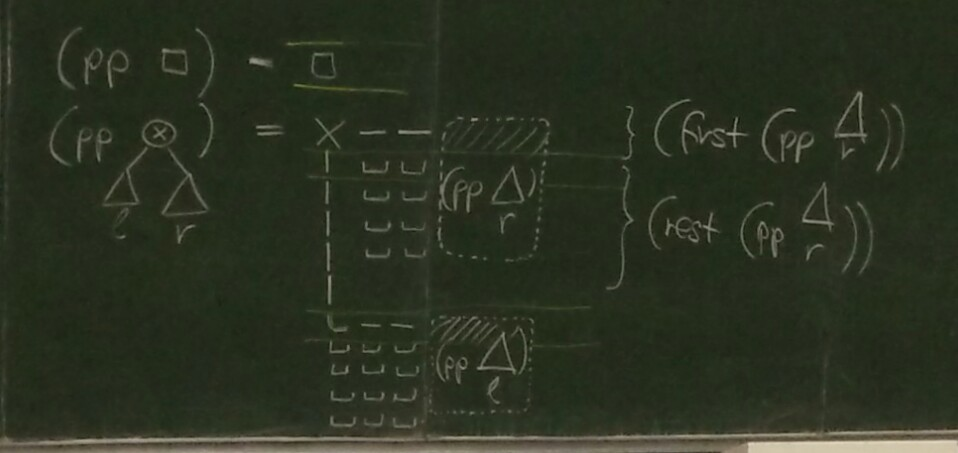
\includegraphics[width=1\textwidth, angle=0]{pretty_printing.jpg}
	\label{fig1}
\end{figure}


Idee: Repräsentiere formatierten String als Liste von Zeilen (Strings).\\
\begin{enumerate}
\item Nutze (string-append ...) um Zeilen-Strings zu definieren. (horizontale Konkatenation).\\
\item Nutze (append ...) um die einzelnen Zeilen zu einer Liste von Zeilen zusammenzusetzen (vertikale Konkatenation).
Erst direkt vor der Ausgabe werden die Zeilen-Strings zu einem auszugebenden String zusammengesetzt. (strings-list $\rightarrow$ string)
\end{enumerate}

\section{Induktion über Binärbäume}
Sei P(t) eine Eigenschaft von Binärbäumen $t \in T(M)$, also \\
\begin{lstlisting}
(: P ((btree-of M) -> boolean))
\end{lstlisting}
Falls P(empty-tree) [Induktionsbasis]\\
und $\forall x \in M$, $l \in T(M), r \in T(M)$:\\
$P(l) \land P(r) \Rightarrow P $ ((make-node l x r))\\
dann $\forall t \in T(M): P(t)$

\subsection{Beispiel:}
Zusammenhang zwischen Grösse (btree-size) und Tiefe (btree-depth) eines Binärbaums t ("ein Baum der Tiefe n enthält mindestens n Knoten und höchstens $2^n - 1$ Knoten"):\\
$P(t) \equiv $ (btree-depth t) $≤$ (btree-size t) $≤ 2^{\textbf{(btree-depth t)}} - 1$\\
Erstes $≤$ trivial. Zweites:\\
Induktionsbasis P(empty-tree):
\begin{lstlisting}
(size empty-tree)
\end{lstlisting}
*$\rightsquigarrow$[depth] 0\\
$= 2^{(0)} -1 \surd$\\
Induktionsschrit: (P (l) $\land P (r) \Rightarrow P$ ((make-node l x r))\\
(size (make-node l x r))\\
$\rightsquigarrow$[size] (size l) + 1 + (size r)\\
$≤$ [I.V.] $2^{\textsl{(depth l)}} - 1 + 1 + 2^{\textsl{(depth r)}} -1$\\
$= 2^{(\textsl{depth l})} + 2^{(\textsl{depth r})} -1$\\
$≤ 2$ x max($ 2^{\textsl{(depth l)}} + 2^{\textsl{(depth r)}}$) -1\\
$= 2 \cdot 2^{\textsl{max((depth l), (depthr)}} -1$\\
$= 2^{(1 + \textsl{max((depth l), (depth r))})}$\\

$\leftarrow$[depth] $2^{\textsl{depth((make-node l x r))}} -1 \surd$\\

Wie müsste sich btree-fold, eine fold-Operation für Binärbäume verhalten? Tree transformer für Baum t:

\begin{figure}[ht]
	\centering
  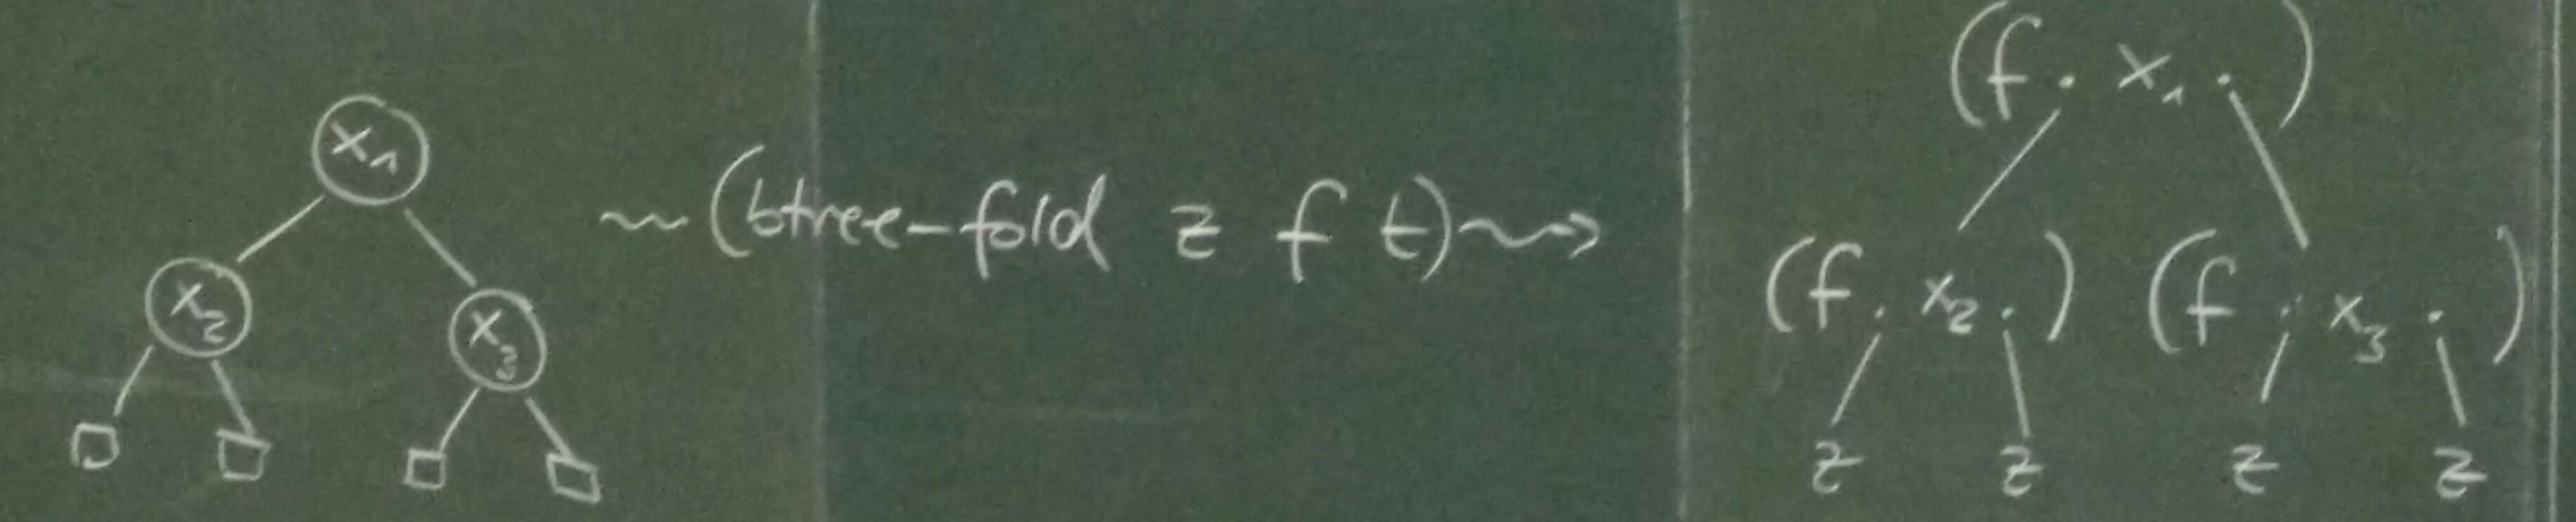
\includegraphics[width=1\textwidth, angle=0]{btree-fold.jpg}
	\label{fig1}
\end{figure}

opku9zfswdefrtgzhujikolpölokijuzhtgrffgtzhujikolpkijuzhtgrftgzhujiklpö [Anmerkung Marvin]

Falte Baum t bzgl. f und z:\\
\begin{lstlisting}
(: btree-fold (%a %b %a -> %a) (btree-of %b) -> %a))
(define btree-fold
	(lambda (z f t)
		(cond ((empty? t) z)
			((node? t) (f (btree-fold z f (node-left-branch t))
					(node-label t)
					(btree-fold z f (note-right-branch t))))))
\end{lstlisting}


\chapter{Fortsetzung Bäume (btree-fold) - 9.7.}
Bestimme die Markierung Lm (left most) links-aussen im Baum t (oder empty, falls t leer ist).\\

(leftmost (x) $\square$ ) = (list x)\\
(leftmost (x) $\Delta$) = (leftmost $\Delta$)\\
Hinweis:\\
- Nutzt die leere Liste (empty) als Fehlerindikator (insbesondere kein Abbruch mit violation)\\
(Prinzip: "Replacing Failure by a list of successes", Philip Wadler)\\
\begin{lstlisting}
(: leftmost ((btree-of %a) -> (list-of %a)))
(check-expect (leftmost empty-tree) empty)
(check-expect (leftost t1) (list 1))
(check-expect (leftost t2) (list 2))

(define leftmost
	(lambda (t)
		(btree-fold empty
				(lambda (l1 x l2) (if (empty? l1)
							(list x)
							l1))
				t)))
\end{lstlisting}


\textbf{Rechtstiefe Bäume und Listen sind isomorph (gleichgestaltig)}\\
Beweis: $f \circ f^{-1} =$ id\\
\begin{lstlisting}
(list->btree (btree->list x))
(right-deep? btree-fold ->  Tuete Gummibaerchen)
\end{lstlisting}

\section{Tiefendurchläufe (depth-first-traversals)}
Ein Tiefendurchlauf (depth-first-traversal) eines Baumes t sammelt die Markierung jedes Knotens n in t auf. Die Markierungen, der Teilbäume L, r des Knotens n = (make-node L x r) werden vor x eingesammelt (Durchlauf zuerst in der Tiefe).\\
Je nachdem, ob x  (a) zwischen, (b) vor, (c) nach den Markierungen von L,r eingeordnet wird, erhält man  ein \\
(a) inorder traversal (xs1 x xs2)\\
(b) preorder traversal (x xs1 xs2)\\
 (c) postorder traversal (xs1 xs2 x).
\begin{lstlisting}
(: inorder ((btree-of %a) -> (list-of %a)))
(define inorder
	(lambda (t)
		(btree-fold empty
					(lambda (xs1 x xs2) (append xs1 (list x) xs2)))
					t)))

\end{lstlisting}
Baumdarstellung eines arithmetischen Ausdrucks \\
Ein Breitendurchlauf (breadth-firrst-traversal ) eines Baumes t sammelt die Markierungen der Knoten ebenenweise von der Wurzel ausgehend auf.\\

\begin{figure}[ht]
	\centering
  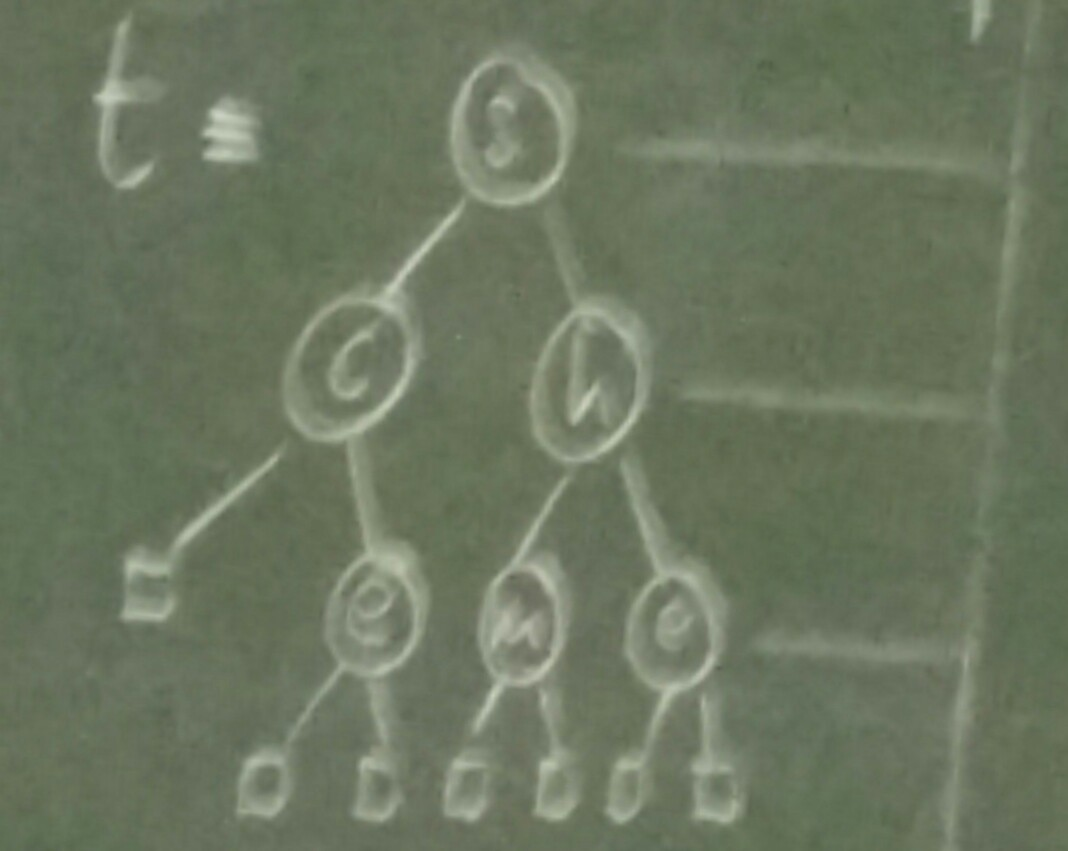
\includegraphics[width=0.33\textwidth, angle=0]{btree-scheme.jpg}
	\label{fig1}
\end{figure}


(levelorder t) $\rightsquigarrow$ (list "s" "c" "h" "e" "m" "e")\\
Idee: Gegeben sei eine Liste ts von Bäumen.
\begin{enumerate}
\item Sammle die Liste der Markierungen der Wurzeln der (nicht-leeren) Bäume in ts auf (= (roots ts) )
\item Bestimme ts' der nicht-leeren Teilbäume der Bäume in ts (= (subtrees ts))
\item Führe (1) rekursiv auf ts' aus.
\item Konkateniere die Listen aus  (1) und (3).
\end{enumerate}

zu Beginn: \\
roots: "s"\\
subtrees: ( (c), (h) )
1. Rekursion: ( (c), (h) )\\
roots: "c" "h"\\
subtrees: ( (e) (m) (e) )\\
2. Rekusion:  ( (e) (m) (e) )\\
roots: "e" "m" "e"
subtress: ( )

\chapter{Zeichencodierungen - 14.07}
bilden Zeichen auf Sequenzen von Bits ab. Derzeit sind Codes \underline{fixer} Länge weit verbreitet.
\begin{itemize}
\item ASCII (Codes 0-127, 7 Bit, American Standard Code for Information Interchange)
\item ISO-8859-1 (Codes 0-255, 8 Bit, 191 lateinische + Steuerzeichen)
\item Unicode (20 Bit, codiert Zeichen 129 aktueller/historischer Sprachen, inklusive Klingon)\\
Beispiel: Zeichen '€': 0000 0010 0000 1010 1100 ("$\backslash$020AC")
\end{itemize}
Huffman-Codes nutzen Bitsequenzen variabler Länge.\\
Idee: Zeichen mit hoher Frequenz werden mit weniger Bits codiert, als seltene Zeichen.\\
$\Rightarrow$ Datenkompression\\
Huffman-Codes sind Binärbäume mit markierten Blättern (Knoten haben keine Codierung). \\
Beispiel: Humman-Code für "erdbeermarmelade":
\begin{lstlisting}
              o
             /   \
            o      o
           / \   /  \
          r  o   o  e
             /\ /\
            m a b l 
\end{lstlisting}
Code für Zeichen x Pfad von Wurzel bis Blatt mit Markierung x.
\begin{itemize}
\item Abstieg in linken Teilbaum Bit 0
\item Abstieg in rechten Teilbaum Bit 1
\end{itemize}

\begin{tabular}{|c|c|c|}
\hline 
Zeichen & Frequenz & Code \\ 
\hline 
e & 5 & 11 \\ 
\hline 
r & 3 & 00 \\ 
\hline 
m & 2 & 010 \\ 
\hline 
a & 2 & 011 \\ 
\hline 
d & 2 & 101 \\ 
\hline 
b & 1 & 1000 \\ 
\hline 
l & 1 & 1001 \\ 
\hline 
\end{tabular} \\
\pagebreak

Huffman-Codes sind präfixfrei.: alle Bits eines bestimmten Zeichens sind niemals Präfix eines anderen Zeichens $\Rightarrow$ eindeutige Decodierung.

$11 | 00 | 101 | 1000 | 11 | 11 | ...  \Rightarrow$ e r d b e e ...\\
Länge 42 Bit, Unicode 320 Bit\\
Einsatz in JPEG, MP3, ZIP, ...\\

\section{Prozeduren zur Huffman-Codierung}
\begin{enumerate}
\item Decodieren einer Bitsequenz (: huff-decode ((huff-tree-of string) (list-of bit) $\rightarrow$ string))
\item Codieren eines Strings: (: huff-encode ((huff-tree-of string) string $\rightarrow$ (list-of bit)))\\
$\forall$ string s: (huff-decode ht (huff-encode ht s)) = s
\item Huffman-Tree für gegebenen Text erstellen: (: huffman-code (string $\rightarrow$ (huff-tree-of string))
\end{enumerate}

Decodieren eines huffman-codierten Strings (= Code von 0/1-Bits)\\
Plan: Baue
\begin{lstlisting}
(: decode ( (huff-tree-of %a) (list-of bit) -> (list-of %a)))
\end{lstlisting}
\begin{enumerate}
\item (decode ht $\square [... bits ...]$) = (make-pair x (decode ht ht [... bits ...])
\item (decode ht $\Delta [ ]$) = empty
\item[3.a)] (decode ht baum [0 bits ...]) = (decode ht linker-teilbaum [... bits ...])
\item[3.b)] (decode ht baum [1 bits ...]) = (decode ht rechter-teilbaum [... bits ...])

??? Neueinstieg an Wurzel des Huffman-Tree $\Rightarrow$ Wurzel des Huffman-Trees als Parameter durchführen.
\end{enumerate}

Huffman-Codierung eines Strings s als Liste von 0/1-Bits\\
Plan:\\
\begin{enumerate}
\item[(a)] Codierung eines Zeichens c:
Suche c mittels einer Tiefensuche von der Wurzel des Huffman-Tree aus. Protokolliere den Pfad beim Abstieg als Liste von 0/1-Bits.\\
Frage: Wie reagieren, wenn die Tiefensuche zu einem Blatt $\ne$ c führt?\\
Idee: Verfolge an innerem Knoten (make-huff-node l r) jeweils linken UND rechten Teilbaum. Suche nach c schlägt fehl in l oder in r. Bei Fehlschlag liefere die leere Bitliste. Beachte:\\
(append empty xs) = xs\\
(append xs empty) = xs\\


\begin{lstlisting}
(: encode ( (huff-tree-of %a) (list-of bit) %a -> (list-of bit)))
				| 	|
		bisheriges Protokoll    Zeichen c
\end{lstlisting}

\begin{enumerate}
\item[1)] (encode $\square$x [... bits ...] c) = empty  ; x $\ne$ c
\item[2)] (encode $\square$c [... bits ...] c) = (reverse  [... bits ...])
\item[3)] (encode baum [... bits ...] c) = (append (encode l-baum [0 bits ...] c) (encode r-baum [1 bits ...] c)
\end{enumerate}

\item[(b)] Codiere Zeichen oder Strings s mit encode (map), verbinde die einzelnen Bit-Listen mit flatten (concat)

\end{enumerate}

\chapter{Fortsetzung Codierung mit Bäumen - 16.07}
(huff-encode $\Delta$ht s) $\rightsquigarrow$ 0111 0100...\\
(huff-decode $\Delta$ht 0111 0100...) $\rightsquigarrow$ s\\

\section{Erstellung eines Huffman-Tree für einen gegebenen Text txt} 
Plan:\\
\begin{enumerate}
\item[(H1)] Stelle Häufigkeit des Vorkommens jedes Zeichens in txt fest. Sortiere in Reihenfolge steigender Häufigkeit. (occurences)\\
Beispiel (occurences "erdbeermarmelade") $\rightsquigarrow$ (list $<$"l",1$>$, $<$"b",1$>$, ... $<$"e",5$>$) Vorkommen $<$i,n$>$ (occur): Ding i (item) kommt mit Häufigkeit n (freq) vor.
\item[(H2)] Baue Huffman-Tree von den Blättern her auf. Initialisiere den Aufbau für Vorkommen $<$i,n$>$ konstruiere $< \square i, n>$.
\item[(H3)] Die beiden Huffman-Trees, die die seltensten Zeichen repräsentieren, stehen am Anfang der Liste.\\
(list $< \square i, n>, <\square j,m>$...)\\
Konstruktion des Huffman-Trees, die diese \underline{Invariante} bewahrt:\\
Iteration: Wiederhole, bis Liste Länge 1 hat\\
\begin{enumerate}
\item[(a)] Fasse Vorkommen $< \Delta l, n>$ und $<\Delta r, m>$ zu einem Vorkommen: $< \Delta
l$-O-$\Delta r, n+m>$
\item[(b)] Sortiere dieses Vorkommen bzgl. Häufigkeit n + m in die Restliste ein.
\end{enumerate}
\item[(H4)] Baum ht in (list $< \Delta ht, n>$) ist der gesuchte Huffman-Tree.

\end{enumerate}

\chapter{DMdA-fortgeschritten - 16.7.}
\begin{itemize}
\item Neues Ausgabeformat in REPL:\\
(list x1 ... xn) $\rightarrow$ (x1 ... xn)\\
empty $\rightarrow$ ()
\item Neuer (struktureller) Gleichheitstest für Werte aller (auch benutzer-definierter) Signaturen:\\
\begin{lstlisting}
(: equal? (%a %b -> boolean))
\end{lstlisting}
\end{itemize}

\section{Quote}
Sei e ein beliebiger Scheme-Ausdruck. Dann liefert (quote e) die Repräsentation von e - e wird \underline{nicht} ausgewertet.
\subsection{Beispiele}
(quote 42) $\rightsquigarrow$ 42\\
(quote "U Tü") $\rightsquigarrow$ "U Tü"\\
Konstante (Literale) repräsentieren sich selbst\\
(quote ( + 40 2)) $\rightsquigarrow$ (+ 40 2) Funktionsapplikation repräsentiert als Liste\\
Abkürzung (quote e) $\equiv$ 'e\\
\subsection{Listennotation in Programmen:}
(list x1 ... xn) $\equiv$ '(x1 .. xn)\\
empty $\equiv$ '()\\
\section{Symbole}
Was ist (first '(* 1 2))? Was sind lambda, x, +, in '(lambda (x) (+ x 1))?\\
$\rightarrow$ Neue Signatur \underline{symbol} zur Repräsentation von Namen in Programmen. Effiziente interne Darstellung (KEINE STRINGS), effizient vergleichbar. Kein Zugriff auf einzelne Zeichen des Symbols.

\section{Operationen:}
\begin{itemize}
\item
\begin{lstlisting}
 (: symbol? (%a -> boolean)) 
 \end{lstlisting}
\end{itemize}
\begin{itemize}
\item
\begin{lstlisting}
(: symbol->string (symbol -> string))
\end{lstlisting}
\end{itemize}

\section{Repräsentation und Auswertung arithmetischer Ausdrücke}
\begin{lstlisting}
		list
\end{lstlisting}
Beispiel: e$\equiv$ '$\overbrace{\textbf{(* (! (+ 1 2)) x)}}$

\begin{lstlisting}
(define arith
	(signature (mixed number 	;Konstanten
			  symbol 	;Variablen
			  (list-of arith))) ; zusammengesetzte Ausdruecke
\end{lstlisting}
Auswertung möglich, wenn Bindung für Symbole (Variablen \underline{und} Operatoren) an Werte gegeben. \underline{Dictionary} (Environment):\\
d1: $\lbrace$ x $\rightarrow$ 3,\\
* $\rightarrow <$procedure: * $>$,\\
+ $\rightarrow <$procedure: + $>$,\\
! $\rightarrow$ fac $\rbrace$\\
$\Rightarrow$ e $\rightsquigarrow$ 18\\

d2: $\lbrace$ x $\rightarrow$ 1,\\
* $\rightarrow <$procedure: * $>$,\\
+ $\rightarrow <$procedure: + $>$,\\
! $\rightarrow$ (lambda (x) (- x)) $\rbrace$\\
$\Rightarrow$ e $\rightsquigarrow$ -3\\

Auswertung eines arithmetischen Ausdrucks e (unter Dictionary d):\\
 ((eval d) e)\\
 konfigurierter Auswerter
 \begin{enumerate}
 \item[(E1)] ((eval d) c) = c ; c Konstante
 \item[(E2)] ((eval $\lbrace x_1 \rightarrow v_1,$ ... , $x_n \rightarrow v_n \rbrace) x_i) = v_i$, ; Xi Variable
 \item[(E3)] Cliffhanger
 \end{enumerate}
\end{document}